\usetikzlibrary{positioning, calc, shapes.misc, shapes.geometric, backgrounds}

\definecolor{red-bert}{RGB}{244,204,204}
\definecolor{blue-bert}{RGB}{201,218,248}
\definecolor{darkblue-bert}{RGB}{80, 129, 188}
\definecolor{yellow-bert}{RGB}{255,242,204}
\definecolor{darkyellow-bert}{RGB}{254,217,102}
\definecolor{green-bert}{RGB}{216,234,210}
\definecolor{gray-bert}{RGB}{243,243,243}

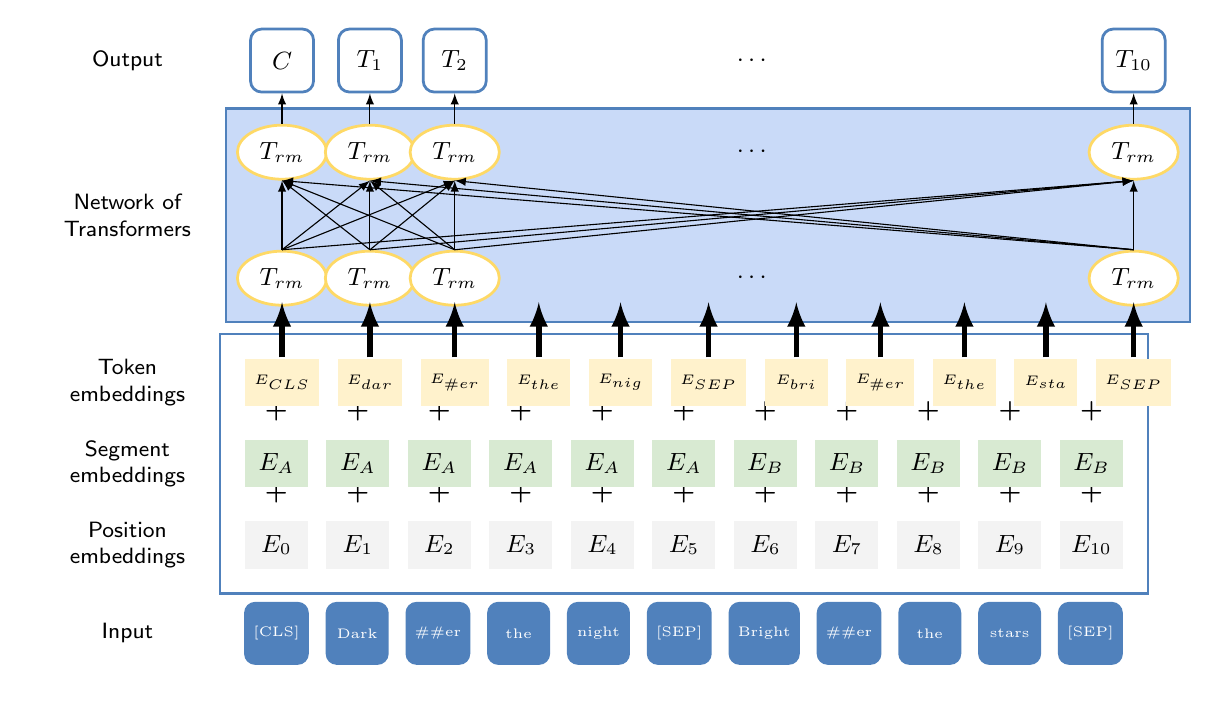
\begin{tikzpicture}[
    node distance=0.2cm,
    >=latex,
    font=\tiny,
    layer-label/.style={text width=2.3cm, minimum height=0.5cm, align=flush center, font=\footnotesize\sffamily},
    token/.style={rectangle, rounded corners, fill=darkblue-bert, text=white, minimum width=8mm, minimum height=8mm},
    posemb/.style={rectangle, fill=gray-bert, minimum height=6mm,minimum width=8mm,line width=1pt, font=\small},
    segemb/.style={rectangle, fill=green-bert, minimum height=6mm,minimum width=8mm,line width=1pt, font=\small},
    toks/.style={rectangle, fill=yellow-bert, minimum height=6mm,minimum width=8mm,line width=1pt, font=\tiny},
    transformer/.style={ellipse, fill=white, draw=darkyellow-bert, minimum height=6mm,minimum width=8mm,line width=1pt, font=\small},
    outnd/.style={rectangle, rounded corners, draw=darkblue-bert, minimum height=8mm,minimum width=8mm,line width=1pt, font=\small},
    ]
]

    \node[layer-label, minimum height=1cm] (input-label) {Input};
    \node[layer-label, above=of input-label] (embedding-label) {Position embeddings};
    \node[layer-label, above=of embedding-label] (encoder-label) {Segment embeddings};
    \node[layer-label, above=of encoder-label] (token-label) {Token embeddings};
    \node[layer-label, above=of token-label, minimum height=3cm] (transformer-label) {Network of Transformers};
    \node[layer-label, above=of transformer-label] (output-label) {Output};

    % The darker the night, the brighter the stars
    \node[token, right=of input-label] (inp-0) {[CLS]};
    \node[token, right=of inp-0] (inp-1) {Dark};
    \node[token, right=of inp-1] (inp-2) {\#\#er};
    \node[token, right=of inp-2] (inp-3) {the};
    \node[token, right=of inp-3] (inp-4) {night};
    \node[token, right=of inp-4] (inp-5) {[SEP]};
    \node[token, right=of inp-5] (inp-6) {Bright};
    \node[token, right=of inp-6] (inp-7) {\#\#er};
    \node[token, right=of inp-7] (inp-8) {the};
    \node[token, right=of inp-8] (inp-9) {stars};
    \node[token, right=of inp-9] (inp-10) {[SEP]};

    % Position embeddings
    \node[posemb, above=of inp-0, right=of embedding-label] (pos-0) {$E_{0}$};
    \node[posemb, right=of pos-0] (pos-1) {$E_{1}$};
    \node[posemb, right=of pos-1] (pos-2) {$E_{2}$};
    \node[posemb, right=of pos-2] (pos-3) {$E_{3}$};
    \node[posemb, right=of pos-3] (pos-4) {$E_{4}$};
    \node[posemb, right=of pos-4] (pos-5) {$E_{5}$};
    \node[posemb, right=of pos-5] (pos-6) {$E_{6}$};
    \node[posemb, right=of pos-6] (pos-7) {$E_{7}$};
    \node[posemb, right=of pos-7] (pos-8) {$E_{8}$};
    \node[posemb, right=of pos-8] (pos-9) {$E_{9}$};
    \node[posemb, right=of pos-9] (pos-10) {$E_{10}$};

    \foreach \i in {0,...,10} {
        \node[above=of pos-\i, yshift=-0.3em] (sum1-\i) {\small \textbf{+}};
    }

    % Segment embeddings
    \node[segemb, above=of pos-0, right=of encoder-label] (seg-0) {$E_{A}$};
    \node[segemb, right=of seg-0] (seg-1) {$E_{A}$};
    \node[segemb, right=of seg-1] (seg-2) {$E_{A}$};
    \node[segemb, right=of seg-2] (seg-3) {$E_{A}$};
    \node[segemb, right=of seg-3] (seg-4) {$E_{A}$};
    \node[segemb, right=of seg-4] (seg-5) {$E_{A}$};
    \node[segemb, right=of seg-5] (seg-6) {$E_{B}$};
    \node[segemb, right=of seg-6] (seg-7) {$E_{B}$};
    \node[segemb, right=of seg-7] (seg-8) {$E_{B}$};
    \node[segemb, right=of seg-8] (seg-9) {$E_{B}$};
    \node[segemb, right=of seg-9] (seg-10) {$E_{B}$};

    \foreach \i in {0,...,10} {
        \node[above=of seg-\i, yshift=-0.3em] (sum1-\i) {\small \textbf{+}};
    }

    % Token embeddings
    \node[toks, above=of seg-0, right=of token-label] (tok-0) {$E_{CLS}$};
    \node[toks, right=of tok-0] (tok-1) {$E_{dar}$};
    \node[toks, right=of tok-1] (tok-2) {$E_{\#er}$};
    \node[toks, right=of tok-2] (tok-3) {$E_{the}$};
    \node[toks, right=of tok-3] (tok-4) {$E_{nig}$};
    \node[toks, right=of tok-4] (tok-5) {$E_{SEP}$};
    \node[toks, right=of tok-5] (tok-6) {$E_{bri}$};
    \node[toks, right=of tok-6] (tok-7) {$E_{\#er}$};
    \node[toks, right=of tok-7] (tok-8) {$E_{the}$};
    \node[toks, right=of tok-8] (tok-9) {$E_{sta}$};
    \node[toks, right=of tok-9] (tok-10) {$E_{SEP}$};

    % rectangle in embeddings
    \begin{scope}[on background layer]
    \draw[darkblue-bert, thick] ($ (tok-0.north west) + (-0.3, 0.3) $) rectangle ($ (pos-10.south east) + (0.3, -0.3) $);
    \end{scope}

    % transformers
    \node[transformer, yshift=-0.8cm] (tm-00) at (transformer-label -| tok-0) {$T_{rm}$};
    \node[transformer, yshift=0.8cm] (tm-01) at (transformer-label -| tok-0) {$T_{rm}$};
    \node[transformer] (tm-10) at (tm-00 -| tok-1) {$T_{rm}$};
    \node[transformer] (tm-11) at (tm-01 -| tok-1) {$T_{rm}$};
    \node[transformer] (tm-20) at (tm-00 -| tok-2) {$T_{rm}$};
    \node[transformer] (tm-21) at (tm-01 -| tok-2) {$T_{rm}$};
    \node[transformer] (tm-n0) at (tm-00 -| tok-10) {$T_{rm}$};
    \node[transformer] (tm-n1) at (tm-01 -| tok-10) {$T_{rm}$};

    % draw cdots
    \node (cdots-1) at ($ .5*(tm-11) + .5*(tm-n1) $) {\small \textbf{$\cdots$}};
    \node (cdots-2) at ($ .5*(tm-10) + .5*(tm-n0) $) {\small \textbf{$\cdots$}};

    % draw rectangle around transformers
    \begin{scope}[on background layer]
    \draw[darkblue-bert, fill=blue-bert, thick] ($ (tm-01.north west) + (-0.3, 0.3) $) rectangle ($ (tm-n0.south east) + (0.3, -0.3) $);

    \end{scope}

    % output
    \node[outnd] (out-0) at (output-label -| tm-01) {$C$};
    \node[outnd] (out-1) at (output-label -| tm-11) {$T_{1}$};
    \node[outnd] (out-2) at (output-label -| tm-21) {$T_{2}$};
    \node[outnd] (out-n) at (output-label -| tm-n1) {$T_{10}$};
    \node (cdots-3) at ($ .5*(out-1) + .5*(out-n) $) {\small \textbf{$\cdots$}};

    % connect token embeddings to first transformers
    \foreach \i in {0,...,10} {
        \draw[->, line width=2pt] (tok-\i) -- ($ (tok-\i.north) + (0, 0.7) $);
    }

    % connect transformers
    \foreach \i in {0,...,2} {
        \foreach \j in {0,...,2} {
            \draw[->] (tm-\i0.north) -- (tm-\j1.south);
        }
    }

    \draw[->] (tm-n0.north) -- (tm-n1.south);
    \draw[->] (tm-00.north) -- (tm-n1.south);
    \draw[->] (tm-10.north) -- (tm-n1.south);
    \draw[->] (tm-20.north) -- (tm-n1.south);
    \draw[->] (tm-n0.north) -- (tm-01.south);
    \draw[->] (tm-n0.north) -- (tm-11.south);
    \draw[->] (tm-n0.north) -- (tm-21.south);

    % connect transformers to output
    \foreach \i in {0,...,2} {
        \draw[->] (tm-\i1.north) -- (out-\i.south);
    }
    \draw[->] (tm-n1.north) -- (out-n.south);
\end{tikzpicture}
